% A simple example showing how to create Harvard style referencing in LaTeX
%
% See http://tex.stackexchange.com/questions/102662/harvard-reference-using-biblatex
% for further discussion
\documentclass[12pt]{report}

\usepackage{hyperref}
\usepackage[english]{babel}
\usepackage[utf8]{inputenc}
\usepackage{ragged2e}
\usepackage{enumitem}

\usepackage{color}
\usepackage{fancyvrb}
\usepackage{pdfpages}
\usepackage{amsmath}
\usepackage{breqn}
\usepackage{csquotes}% Recommended
\usepackage{graphicx}
\usepackage[style=authoryear-ibid,backend=biber]{biblatex}
\usepackage{subcaption}
\usepackage{geometry}
\usepackage{caption}
\usepackage{titlesec}
\usepackage{pgfgantt}
\usepackage{lipsum}


\usepackage{etoolbox}
% BUGFIX FOR NON NUMBERING SECTIONS!!!!
\makeatletter
\patchcmd{\ttlh@hang}{\parindent\z@}{\parindent\z@\leavevmode}{}{}
\patchcmd{\ttlh@hang}{\noindent}{}{}{}
\makeatother

% Chapter number supression
\makeatletter
\def\@makechapterhead#1{%
  \vspace*{50\p@}%
  {\parindent \z@ \raggedright \normalfont
    \ifnum \c@secnumdepth >\m@ne
      %\if@mainmatter
        %\huge\bfseries \@chapapp\space \thechapter
        \Huge\bfseries \thechapter.\space%
        %\par\nobreak
        %\vskip 20\p@
      %\fi
    \fi
    \interlinepenalty\@M
    \Huge \bfseries #1\par\nobreak
    \vskip 40\p@
  }}
\makeatother

\newcommand{\sectionbreak}{\clearpage}
\geometry{margin=2.0cm}

\graphicspath{ {./images/} }
\addbibresource{main.bib}% Syntax for version >= 1.2



% Document
\begin{document}
    
\includepdf[page=-]{cover_page}
    \begin{abstract}
        Localization in robotics refers to the problem of determining the pose of a system.
        This involves the combination of sensor readings and mathematical models of the system in question.
        The sensors used is often tied to the task and environment the system operates in.
        For indoor applications, Global Positioning System (GPS) sensors are unreliable and other sensors must be used.
        In this project we will look at integrating a Local Positioning System (LPS) that uses Trilateration with Ultra-WideBand (UWB) technology.
    \end{abstract}

    \chapter*{Acknowlegdments}
    \lipsum[2-4]

    \chapter*{Nomenclature}
    \begin{itemize}[label={}]
        \item UAV - Unmanned Aerial Vehicle.
        \item GPS - Global Positioning System.
        \item LPS - Local Positioning System.
        \item FCU - Flight Controller Unit.
        \item UWB - Ultra-WideBand.
        \item TOF - Time of Flight.
        \item PSoC - Programmable System on Chip.
    \end{itemize}
    \tableofcontents

        \chapter{Introduction}\label{ch:introduction}
%    test ~\parencite{pozyx2018pozyx}
%    \lipsum[2-4]
    In recent years Unmanned aerial vehicle(UAV) usages has grown exponentially becoming common in industry and households~\parencite{custers2016drones}.
    A major part of UAV applications is their ability to localise themselves in the given environment with acceptable precision and accuracy.
    This is a common requirement in any robotic system but UAV's are often limited by strict payload requirements and therefore have to rely on sensors that are lightweight and robust.
    ~\textcite{ardupilotadvanced} gives a good summary of physical components that are used in various vehicles but a UAV system, specifically, a quadrotor system cab be summarised as follows:
    \begin{itemize}
        \item Rotor build - This section contains parts that should be researched based on the size and physical requirements of the drone.
        These include: brushless motors, electronic speed controllers, frame size.
        \item Flight controller unit(FCU) - This acts as the mother board and brain of the quadrotor system.
        It collates data from various sensors, sends commands to the motors and if there is a companion computer is attached collects and sends data to it.
        Commercial FCU's contain the various control systems and laws required for stable flight and movement.
        Most have an array of sensors built in.
        \item Sensors - These vary from from inertial, positioning, barometric and camera.
        Aside from inertial and barometric sensors that are present in most FCU's, sensors are chosen based on the environment and use case of the system.
        \item Companion computer - In some cases higher level processing is required by the system to execute autonomy and a secondary computer is used to do this.
        \item Transmitter and Receiver - This is used to implement manual control over the drone by a user.
    \end{itemize}
    Further delving into the sensors, we can classify UAV's based on their operating environment, indoors or outdoors.
    These give rise to two forms of localisation and navigation systems:
    \begin{itemize}
        \item Global Positioning Systems (GPS) - As the name suggests this setup uses GPS as well as other sensors.
        \item GPS-denied - These systems do not have access to GPS due to their operating environment.
    \end{itemize}
    In outdoor applications GPS provides a reliable and fairly accurate way to localise with use of several other sensors.
    However, indoor applications are denied the benefits of GPS and often must use other sensors for the task of localisation.
    Utilizing a similar concept of triangulation used by GPS a local positioning system(LPS) can be used for indoor environments.
    ~\textcite{pozyx2018pozyx} has developed a commercial system that utilizes Ultra-WideBand technology(UWB) with a bandwidth of $~\approx 500MHz$.

    With indoor environments users have more control of the environment so a LPS can create a feasible solution for indoor localisation for UAV's/robots operating there.
    The core idea of this research would be to integrate a commercial LPS directly into an existing FCU to produce accurate position estimates that can be used for autonomy.
    The measurements from the LPS would then be transformed into observations of the state of the UAV and fused with other observations from other sensors.
    This fused pose estimate would then be fed into the companion computer for off-board processing.
    \begin{figure}[h!]
        \centering
        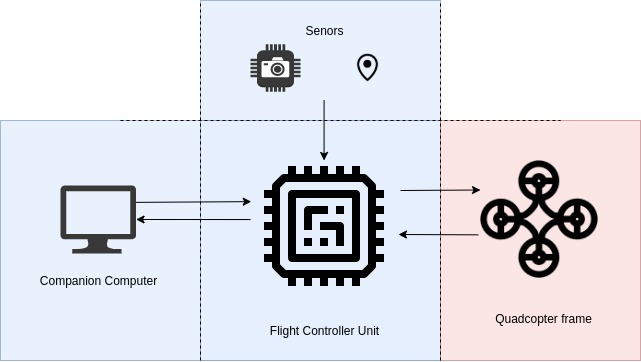
\includegraphics[scale=.65]{drone_setup}
        \caption{The typical setup for an autonomous UAV.}
        \label{fig:ds}
    \end{figure}

    Figure:~\ref{fig:ds} shows a typical setup for UAV.
    Parts of the system highlighted in blue represent systems that would be worked on during the course of this research.
    The idea is that the system being designed should provide localisation data which should be independent of the rotor build.
    These will be further scoped in the upcoming sections but it will involve doing a quality exercise of the LPS tp determine measurement uncertainty and limitations,
    writing additions or modifying the firmware of the FCU to integrate the LPS and setting up the piplines for a companion computer to receive the pose estimates and use them.



    % Give intro to LPS, proposed setup and then plan to complete


    \section{Aims \& Objectives}\label{sec:aims_objs}

    In ~\ref{ch:intro} we briefly touched on what would be addressed over the course of this research.
Expanding on that, the research would entail the use of the commercial version of an UWB sensor for positioning from ~\cite{pozyx2018pozyx}.
At a high level the project and be split into three modules that must be researched, unit tested and finally integrated.
Figure ~\ref{fig:ds} highlights the major systems within the project and are as follows:
\begin{itemize}
    \item The Pozyx LPS providing measurements that will be used in localisation.
    \item A flight controller collating fusing various observations from sensors to provide a pose estimate.
    \item A companion computer to visualise and utilise the pose information in a meaningful manner.
\end{itemize}

From these systems and the overall aim of indoor localisation the following objectives were created:
\begin{itemize}
    \item Evaluation and qualitative analysis of the LPS, documentation limitations from previous done work and current physical setups as well as compare with other ranging standards.
    \item Based on the qualitative analysis and experiments determine the best configuration in a household to place the anchors for the system.
    \item Use the incoming data from the sensors to produce a suitable measurement/observation model for the pose of the system.
    \item Relay the data to a flight controller unit via a suitable hardware interface.
    \item Delve into the firmware of the flight controller and integrate the sensor readings into the codebase.
    \item Apply sensor fusion algorithms to provide pose estimates either onboard the flight controller or through some other medium.
    \item Evaluate pose estimates in various scenarios to see if they are viable for use.
\end{itemize}

All of these objectives can be completed without flying the UAV autonomously.
Given the current situation and time-frame it was determined that setting up the pipelines to visualise the localisation in realtime from the companion computer is adequate for the last objective.
Furthermore, with the autonomous flight being out of scope of this project much of the work fell into software engineering to achieve the overall aim.
Broadly, this means delving into the software libraries and interfaces for the Pozyx sensor, modifying and making additions to the Ardupilot flight stack to integrate the Pozyx sensor with the FCU,
and finally digging into the MAVLINK protocol and libraries to use the pose estimates on a Raspberry Pi 3 Model B+ PSoC.
To achieve these objectives a solid software engineering aproach would need to be applied with familiarity of Python and C++ programming languages.
Additionally, pose estimates should be evaluated under various tests which are not ideal for the LPS system to see how robust the estimator is.
A further limitation may be that due to the lack of accessible hardware and the scope of this research if pose estimates are unavailable from the flight controller a similar setup should be designed in order to closely emulate the results expected from the flight controller unit.



    \chapter{Background Research}\label{ch:background-research}
    \lipsum[2-4]

    \chapter{Literature Review}\label{ch:literature-review}
    \lipsum[2-5]
    \printbibliography[heading=bibintoc]

\end{document}
